\documentclass{beamer}
\usetheme{Madrid}
\usepackage{graphicx,animate} % for \animategraphics

\title{Brief \LaTeX \ Review}
\centering
\date{\today}
\begin{document}

\begin{frame}
	\titlepage
\end{frame}

\begin{frame}{Outline}
	\tableofcontents
\end{frame}

\section{What is \TeX?}
\begin{frame}{What is \TeX?}
\begin{definition}
	TeX is a typesetting system (or a "formatting system"). It was designed and mostly written by Donald Knuth and released in 1978.
\end{definition}
\footnotesize
Donald Ervin Knuth is a professor emeritus at Stanford University. He is the 1974 recipient of the ACM Turing Award.\\
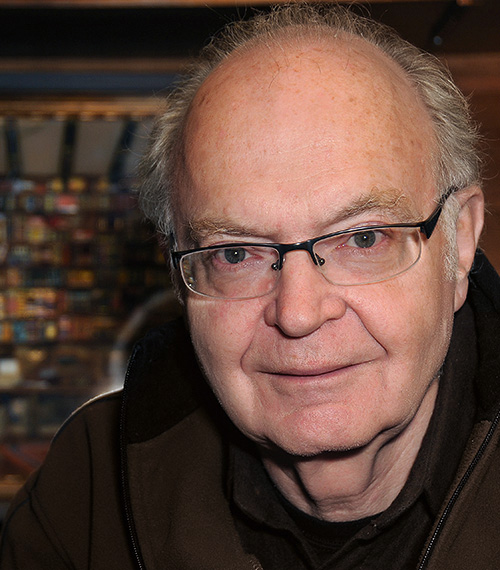
\includegraphics[width=0.20\textwidth]{knuth.jpg}

\end{frame}

\section{What is \LaTeX?}
\begin{frame}{What is \LaTeX?}
\begin{definition}
	\LaTeX, which is pronounced «Lah-tech» or «Lay-tech»  is a \textbf{document preparation system} for high-quality typesetting. It is most often used for medium-to-large technical or scientific documents but it can be used for almost any form of publishing.
\end{definition}
	\LaTeX\ is not a program by itself; it is a language.
\end{frame}

\section{Installation of \LaTeX}
\begin{frame}{Installation of \LaTeX}
	Using \LaTeX\ requires a bunch of tools. TeX Distributions help the user in this way, in that it is a single step installation process that provides (almost) everything.\footnote{\href{https://en.wikibooks.org/wiki/LaTeX/Installation}{https://en.wikibooks.org/wiki/LaTeX/Installation}}\\
	What you need are:
	\begin{enumerate}
		\item \hyperlink{texdistros}{\textbf{TeX distribution}}
		\item \hyperlink{texteditors}{\textbf{Text editor}}
		\item PDF viewer
	\end{enumerate}
	All these can be installed on Windows, Linux, MacOS and many other platforms. \\
\end{frame}

\subsection{TeX distributions}\hypertarget{texdistros}{}
\begin{frame}{TeX distributions}
	In general, we have:
	\begin{itemize}

		\item TeX Live \\
		\href{https://www.tug.org/texlive/quickinstall.html}{\beamerbutton{Installation guidelines for TeX Live}}
		
		\item MiKTeX \\
		\href{https://miktex.org/download}{\beamerbutton{Download page for MiKTeX}}
		
		\item MacTeX (for Mac) \\
		\href{https://www.tug.org/mactex/mactex-download.html}{\beamerbutton{Installation guidelines for MacTeX}}
	\end{itemize}
\end{frame}

\subsection{\LaTeX\ Editors}\hypertarget{texteditors}{}
\begin{frame}{\LaTeX\ Editors}
\begin{enumerate}
    \item For offline editing (not an exhaustive list): \\
	\begin{itemize}
		\item \href{http://www.xm1math.net/texmaker/}{\beamerbutton{Texmaker}}
		\item \href{https://www.texstudio.org/}{\beamerbutton{TeXstudio}}
	\end{itemize}
    \item For online editing (not exhaustive): \\
	\begin{itemize}
		\item \href{https://www.sharelatex.com/}{\beamerbutton{sharelatex.com}}
		\item \href{https://www.overleaf.com/}{\beamerbutton{overleaf.com}}
	\end{itemize}
\end{enumerate}
\end{frame}

\section{\LaTeX Features}
\begin{frame}{\LaTeX Features}
	\begin{itemize}
		\item Typesetting journal articles, technical reports, books, and slide presentations.
        \item Control over large documents containing sectioning, cross-references, tables and figures.
        \item Typesetting of complex mathematical formulas.
        \item Advanced typesetting of mathematics with AMS-LaTeX.
        \item Automatic generation of bibliographies and indexes.
        \item Multi-lingual typesetting.
        \item Inclusion of artwork, and process or spot colour.
        \item Using PostScript or Metafont fonts.
	\end{itemize}
\end{frame}


\end{document}
